
\documentclass[a4paper, 11pt]{beamer}
\usepackage[utf8]{inputenc}
\usepackage[T1]{fontenc}
\usepackage{amsmath}
\usepackage{enumerate}
\usepackage{dblfloatfix}
\usepackage{hyperref}


\newcommand{\source}[1]{\begin{textblock*}{4cm}(8.7cm,8.6cm)
    \begin{beamercolorbox}[ht=0.5cm,right]{framesource}
        \usebeamerfont{framesource}\usebeamercolor[fg]{framesource} Source: {#1}
    \end{beamercolorbox}
\end{textblock*}}

\usetheme{Warsaw}
\usecolortheme{beaver}
\begin{document}

\setbeamertemplate{caption}{\raggedright\insertcaption\par}

\title{Impact of network topology on opinion dynamics in a bounded confidence model}
\author{Artur Przybyłek}
\institute{supervisor: Dr hab. Janusz Szwabiński}
%
\begin{frame}%
\titlepage
\end{frame}
%
\begin{frame}
\frametitle{Presentation plan}
\tableofcontents
\end{frame}

\section{Introduction}

\subsection{Network topologies}

\begin{frame}
\frametitle{Network topologies and their parameters}
\begin{itemize}

	\item complete graph
	\begin{itemize}
		\item $n$: number of agents
	\end{itemize}

	\item Watts--Strogatz
	\begin{itemize}
		\item $n$: number of agents
		\item $k$: number of neighbours for each agent
		\item $p$: probability of changing agent's neighbour
	\end{itemize}
	
		\item Barabasi--Albert
	\begin{itemize}
		\item $n$: number of agents
		\item $m$: number of new connections made for each attached agent to network
	\end{itemize}
	
\end{itemize}
\end{frame}

\begin{frame}
\frametitle{Complete graph}
\begin{figure}[H]
		\centering
		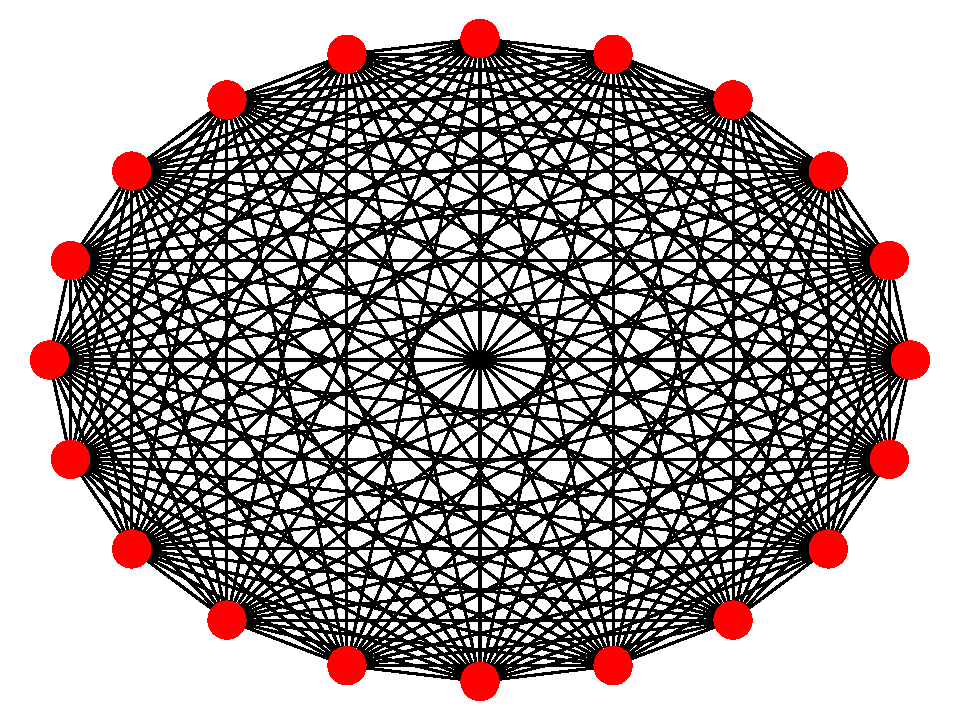
\includegraphics[width=.6\textwidth]{/home/arti/studia/python/praca_magisterska/plots/net_cg_20.pdf}
		\caption{Example network with complete graph topology ($n=20$)}
\end{figure}
\end{frame}

\begin{frame}
\frametitle{Watts--Strogatz}
\begin{figure}[H]
		\centering
		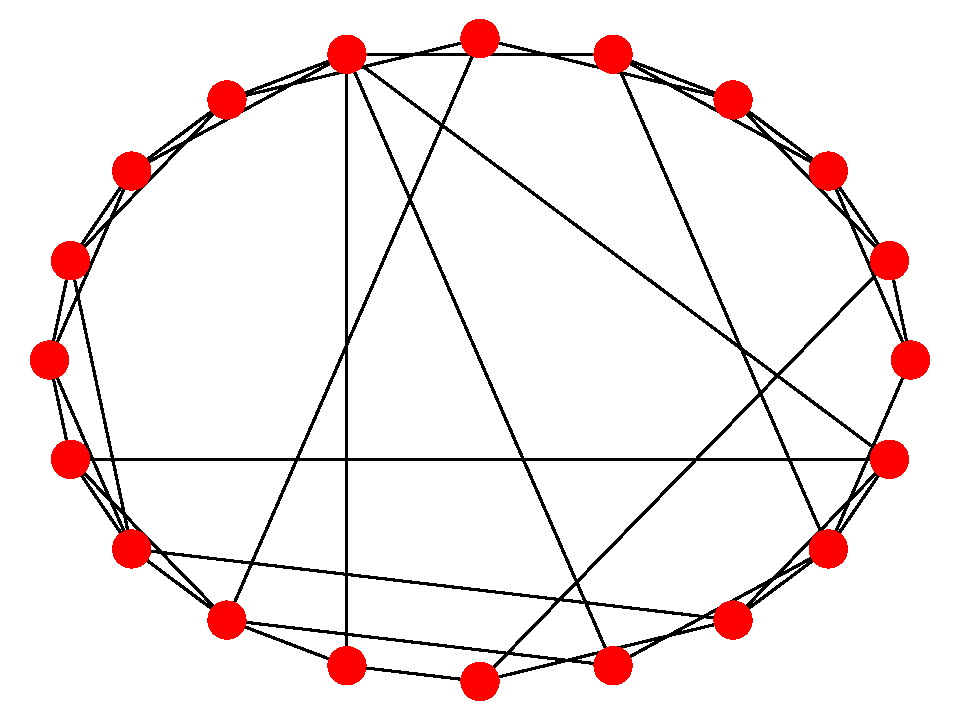
\includegraphics[width=.6\textwidth]{/home/arti/studia/python/praca_magisterska/plots/net_ws_4_0,25.pdf}
		\caption{Example network with Watts--Strogatz topology ($n=10$, $k=4$, $p=0.25$)}
\end{figure}
\end{frame}

\begin{frame}
\frametitle{Barabasi--Albert}
\begin{figure}[H]
		\centering
		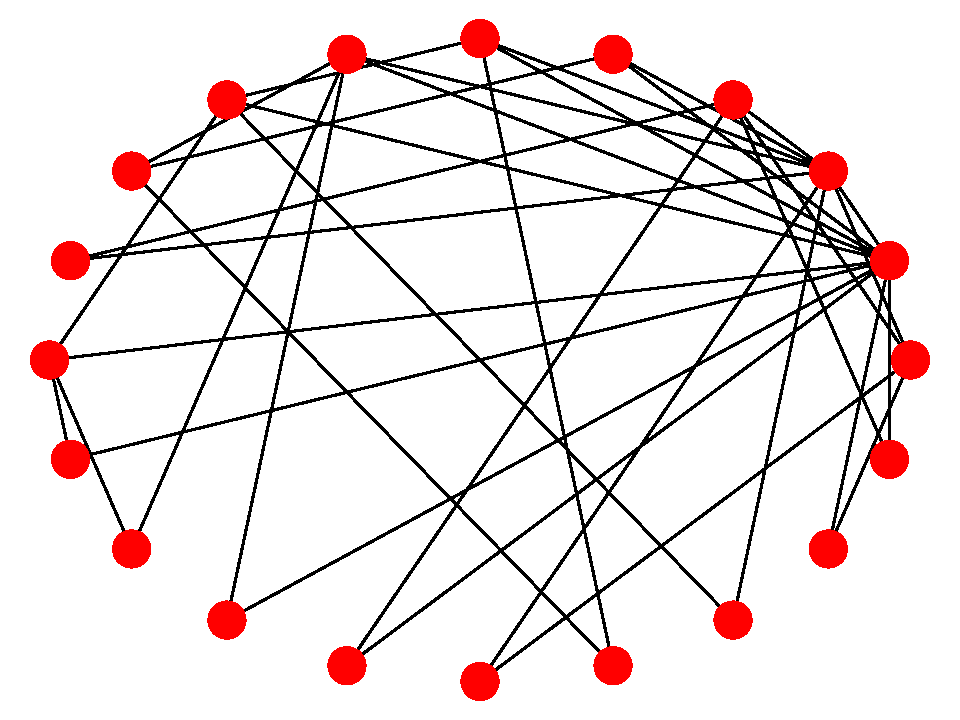
\includegraphics[width=.6\textwidth]{/home/arti/studia/python/praca_magisterska/plots/net_ba_20_2.pdf}
		\caption{Example network with Barabasi--Albert topology ($n=10$, $m=2$)}
\end{figure}
\end{frame}

\subsection{Bounded Confidence model}
\begin{frame}
\frametitle{Assumptions}
\begin{itemize}
	\item agent's opinion can be expressed as a number in interval \textbf{$[0, 1]$} 
	\item agent influence other's opinion only if their opinions are similiar
	\item \textbf{confidence level} is parameter which regulates how much agents take into account others opinions
\end{itemize}
\end{frame}


\begin{frame}
\frametitle{Model}
Let $\epsilon$ be a confidence level and $T={0,1,2,\ldots}$ be a time space of evolution of opinions. Then, opinion of $i$--th agent at time $t+1$ can be expressed by the following equation:
\begin{equation}
x_i(t+1) = \left| I(i, x_i(t)) \right|^{-1} \sum_{j \in I(i, x_i(t))} {x_j(t)},
\label{bc}
\end{equation} 
where $x_i(t)$ is opinion of $i$-th agent at time $t$ and $I(i, x_i(t))$ is the set of neighbours of $i$-th agent for which following equation holds: $\left| x_i(t) - x_j(t) \right| < \epsilon$.
\end{frame}






\section{Simulations}

\subsection{Methodology}

\begin{frame}
\frametitle{Subjects of studies}
\begin{itemize}
	\item{final opinions distribution}
	\item{fragmentation of opinions}
	\item{impact of confidence level on reaching consensus}
	\item{relaxation time}
\end{itemize}
\end{frame}

\begin{frame}
\frametitle{Simulations methodology}
\begin{itemize}
	\item initial opinions randomly distributed from $\mathcal{U}(0,1)$ distribution
	\item in one time step: $n$--times randomly choose agent and change his opinion due to equation (\ref{bc})
	\item{changing only one network parameter and comparing results}
	\item{average results after 100 simulations for given set of parameters}
	\item{consensus state when 80\% of agents share their opinion}
	\item{number of clusters: clusters of agents sharing opinion, with it's size being at least 10\% size of the biggest cluster}
\end{itemize}
\end{frame}

\subsection{Single runs}

\begin{frame}
\frametitle{Single runs: Complete graph}
\begin{figure}[H]
		\centering
		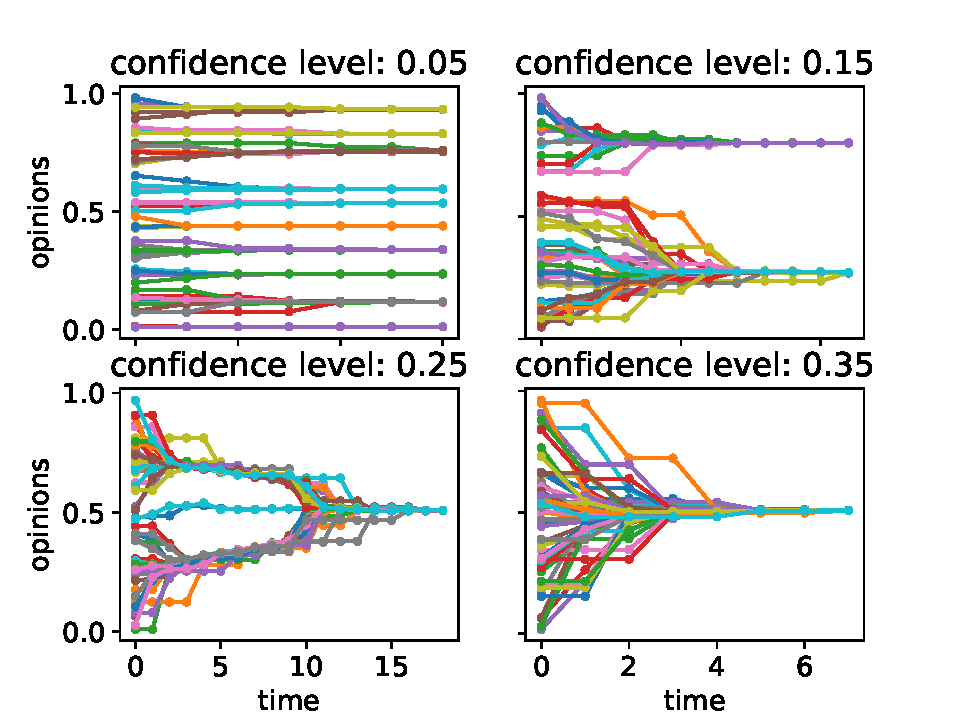
\includegraphics[width=.6\textwidth]{/home/arti/studia/python/praca_magisterska/plots/single_cg_50.pdf}
		\caption{Single simulations on complete graph topology ($n=50$)}
\end{figure}
\end{frame}

\begin{frame}
\frametitle{Single runs: Watts--Strogatz}
\begin{figure}[H]
		\centering
		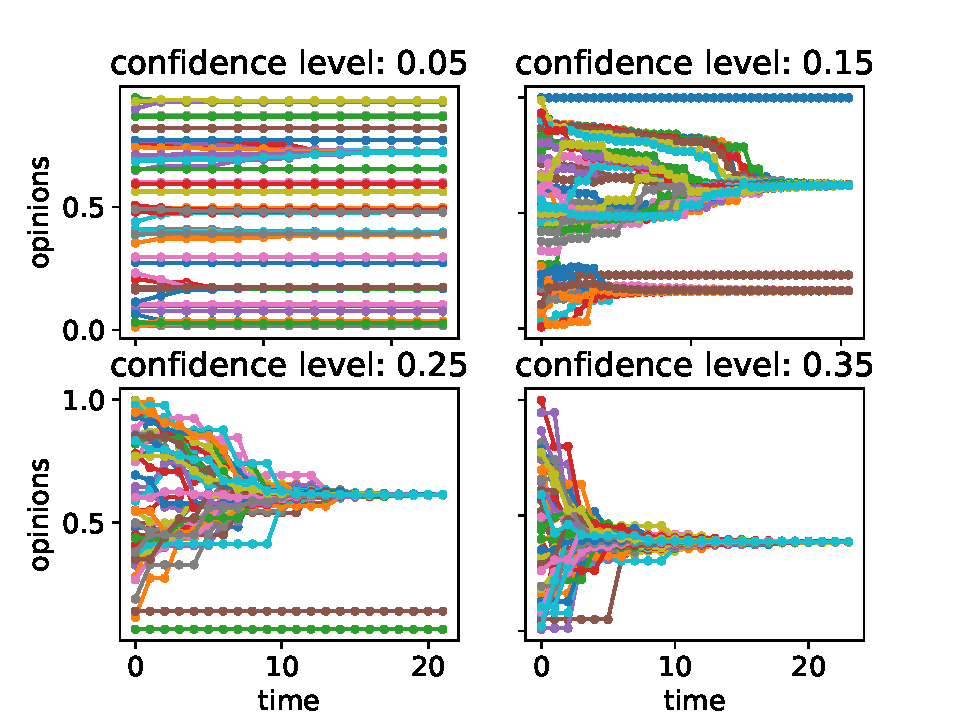
\includegraphics[width=.6\textwidth]{/home/arti/studia/python/praca_magisterska/plots/single_ws_50_10_0,3.pdf}
		\caption{Single simulations on Watts--Strogatz topology ($n=50$, $k=10$, $p=0.3$)}
\end{figure}
\end{frame}

\begin{frame}
\frametitle{Single runs: Barabasi--Albert}
\begin{figure}[H]
		\centering
		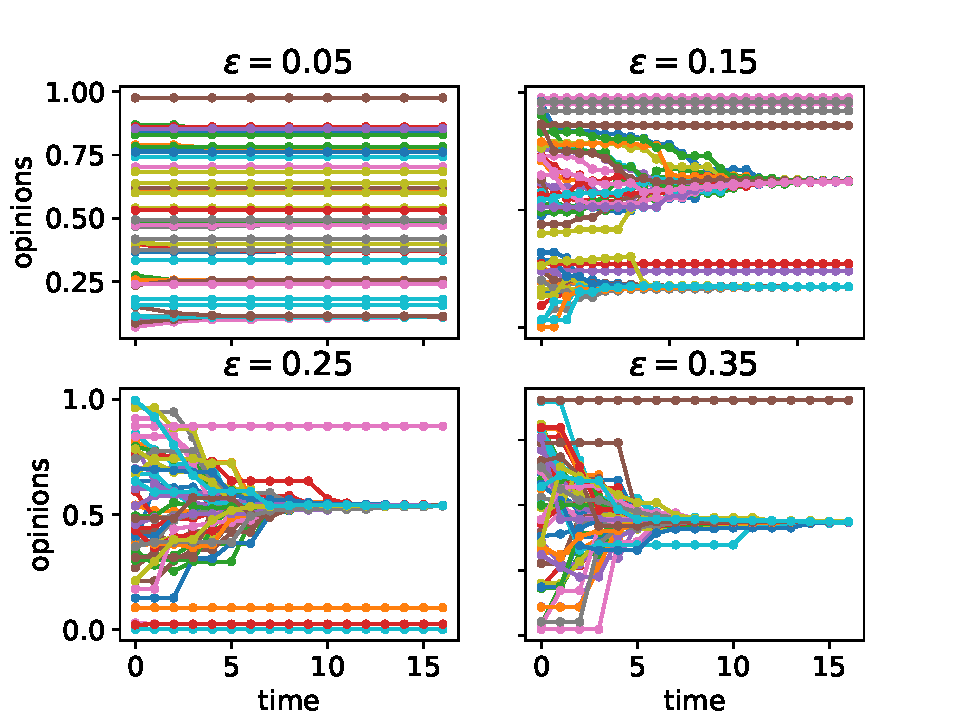
\includegraphics[width=.6\textwidth]{/home/arti/studia/python/praca_magisterska/plots/single_ba_50_4.pdf}
		\caption{Single simulations on Barabasi--Albert topology ($n=50$, $m=4$)}
\end{figure}
\end{frame}

\section{Results}

\subsection{Final opinions distribution}

\begin{frame}
\frametitle{Final opinions distribution: Complete graph}
\begin{figure}[H]
		\centering
		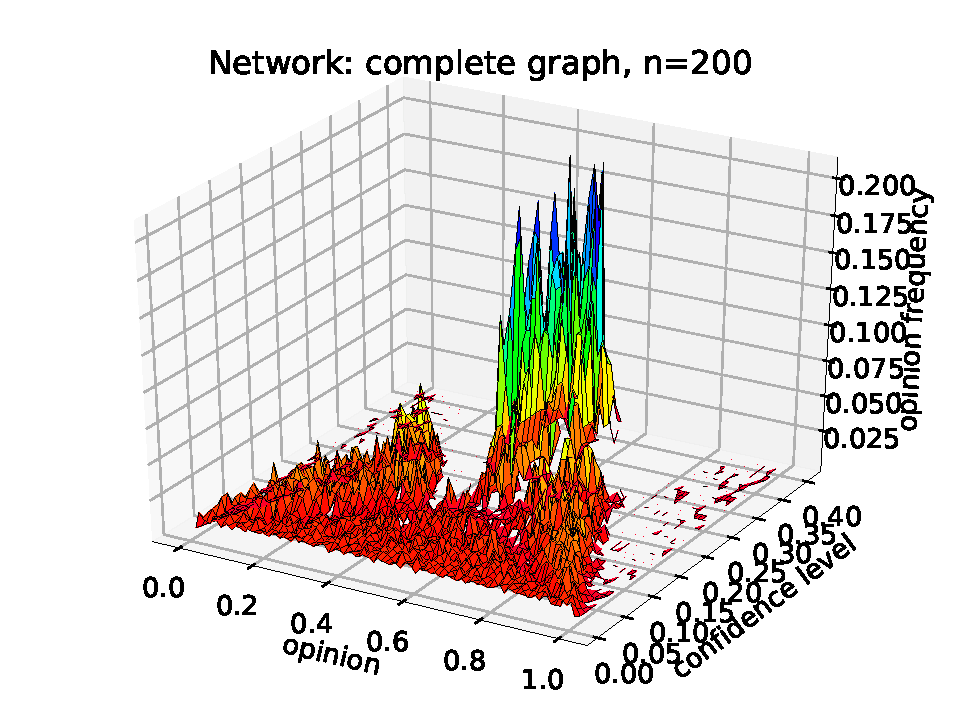
\includegraphics[width=.6\textwidth]{/home/arti/studia/python/praca_magisterska/plots/avg_freq_cg_200.pdf}
		\caption{Average frequency of opinions: complete graph ($n=200$)}
\end{figure}
\end{frame}

\begin{frame}
\frametitle{Final opinions distribution: Watts--Strogatz}
\begin{figure}[H]
		\centering
		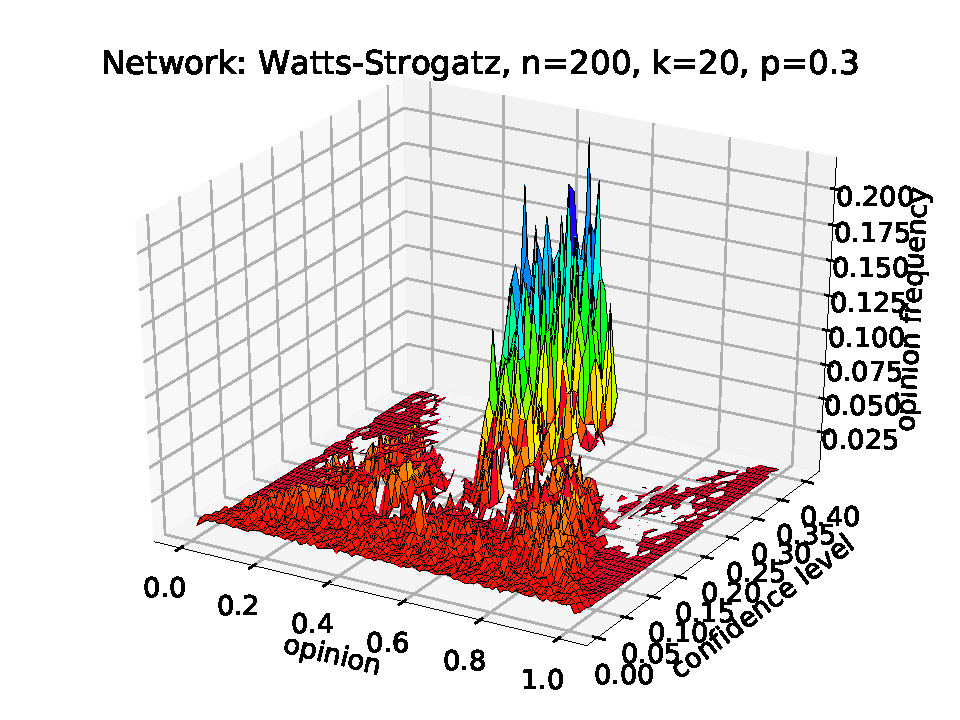
\includegraphics[width=.6\textwidth]{/home/arti/studia/python/praca_magisterska/plots/avg_freq_ws_200_20_0,3.pdf}
		\caption{Average frequency of opinions: Watts--Strogatz ($n=200$, $k=20$, $p=0.3$)}
\end{figure}
\end{frame}


\begin{frame}
\frametitle{Final opinions distribution: Barabasi--Albert}
\begin{figure}[H]
		\centering
		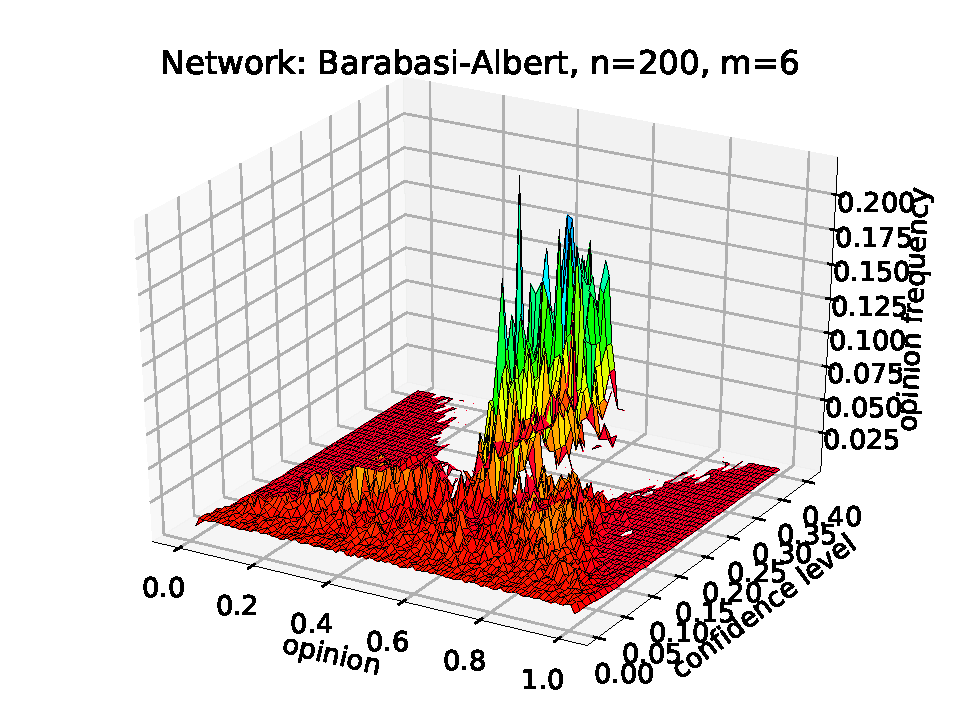
\includegraphics[width=.6\textwidth]{/home/arti/studia/python/praca_magisterska/plots/avg_freq_ba_200_6.pdf}
		\caption{Average frequency of opinions: Barabasi--Albert ($n=200$, $m=6$)}
\end{figure}
\end{frame}


\subsection{Fragmentation of opinions}

\begin{frame}
\frametitle{Fragmentation of opinions}
	\begin{figure}[ht]
		\begin{minipage}[b]{0.45\linewidth}
            \centering
            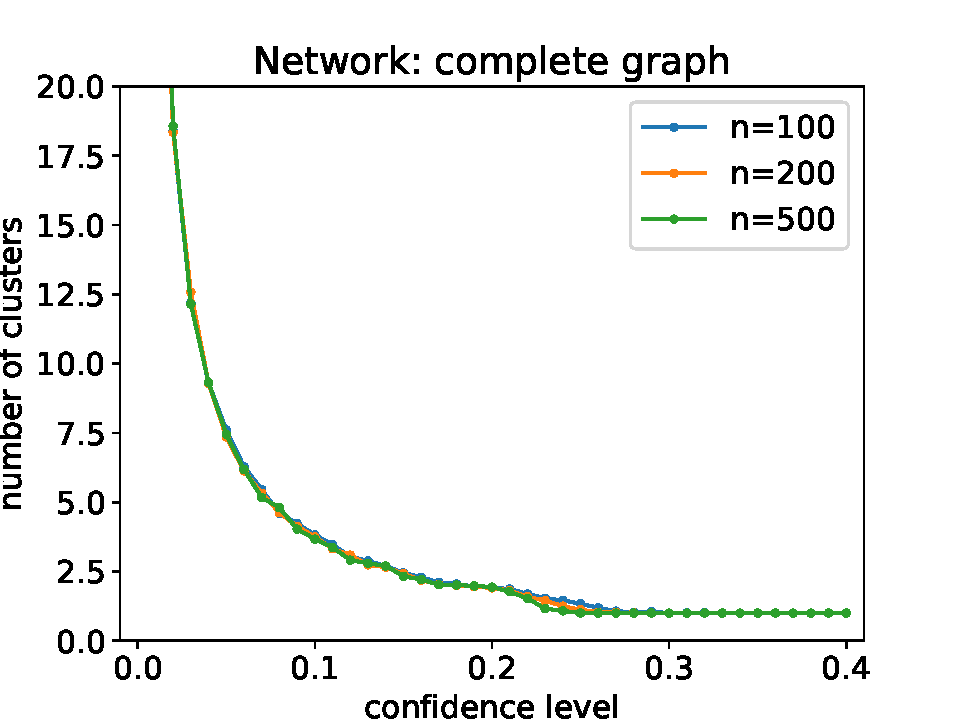
\includegraphics[width=\textwidth]{/home/arti/studia/python/praca_magisterska/plots/groups10_completegraph.pdf}
            \caption{Complete graph: various $n$}
        \end{minipage}
        \hspace{0.5cm}
        \begin{minipage}[b]{0.45\linewidth}
            \centering
            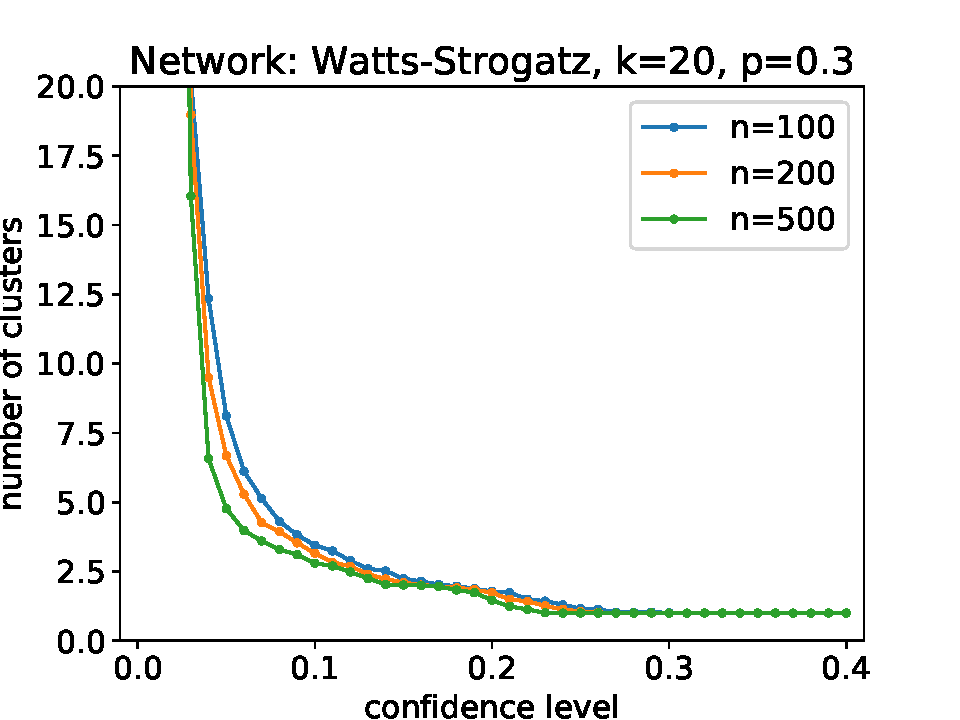
\includegraphics[width=\textwidth]{/home/arti/studia/python/praca_magisterska/plots/groups10_Watts-Strogatz_k=20_p=0_3.pdf}
            \caption{Watts--Strogatz: various $n$}
        \end{minipage}
    \caption{Average number of clusters}
    \end{figure}
\end{frame}

\begin{frame}
\frametitle{Fragmentation of opinions}
	\begin{figure}[ht]
		\begin{minipage}[b]{0.45\linewidth}
            \centering
            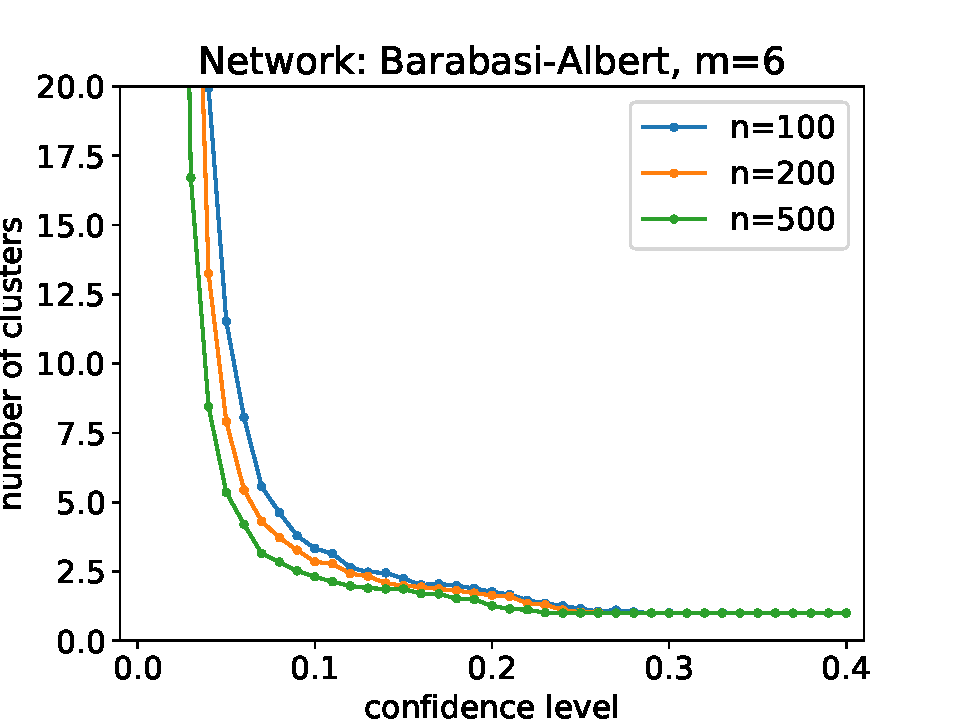
\includegraphics[width=\textwidth]{/home/arti/studia/python/praca_magisterska/plots/groups10_Barabasi-Albert_m=6.pdf}
            \caption{Barabasi--Albert: various $n$}
        \end{minipage}
        \hspace{0.5cm}
        \begin{minipage}[b]{0.45\linewidth}
            \centering
            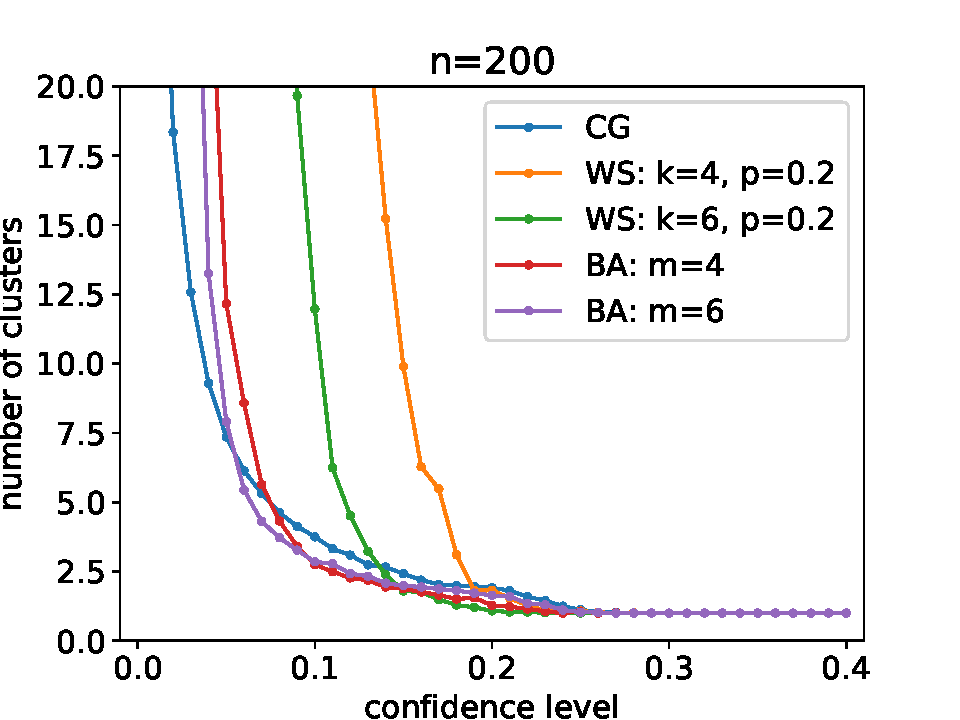
\includegraphics[width=\textwidth]{/home/arti/studia/python/praca_magisterska/plots/groups10_various.pdf}
			\caption{Various networks}
        \end{minipage}
    \caption{Average number of clusters}
    \end{figure}
\end{frame}



\subsection{Impact of confidence level on reaching consensus}

\begin{frame}
\frametitle{Consensus}
	\begin{figure}[ht]
		\begin{minipage}[b]{0.45\linewidth}
            \centering
            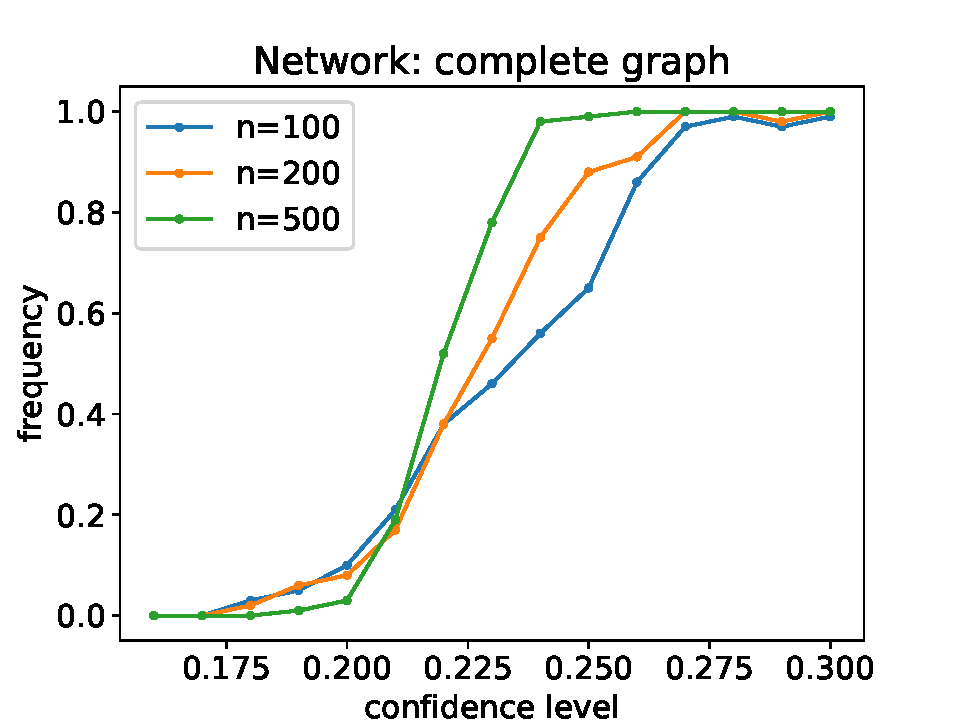
\includegraphics[width=\textwidth]{/home/arti/studia/python/praca_magisterska/plots/freq_consensus_cg.pdf}
            \caption{Complete graph: various $n$}
        \end{minipage}
        \hspace{0.5cm}
        \begin{minipage}[b]{0.45\linewidth}
            \centering
            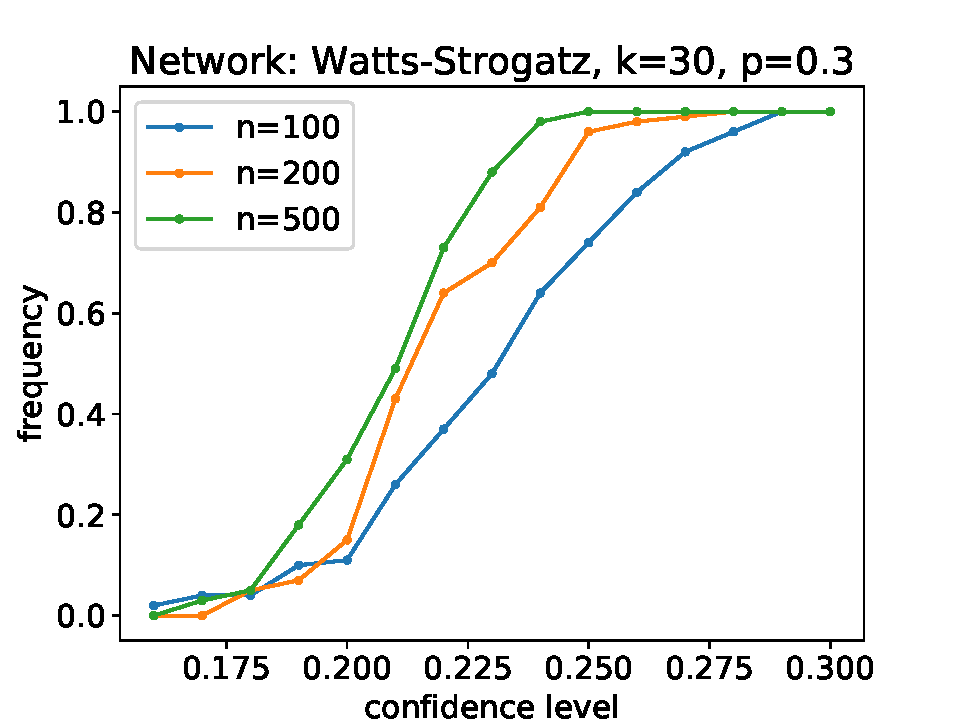
\includegraphics[width=\textwidth]{/home/arti/studia/python/praca_magisterska/plots/freq_consensus_ws_k=30_p=0,3.pdf}
			\caption{Watts--Strogatz: various $n$}
        \end{minipage}
    \caption{Frequency of reaching consensus}
    \end{figure}
\end{frame}

\begin{frame}
\frametitle{Consensus}
	\begin{figure}[ht]
		\begin{minipage}[b]{0.45\linewidth}
            \centering
            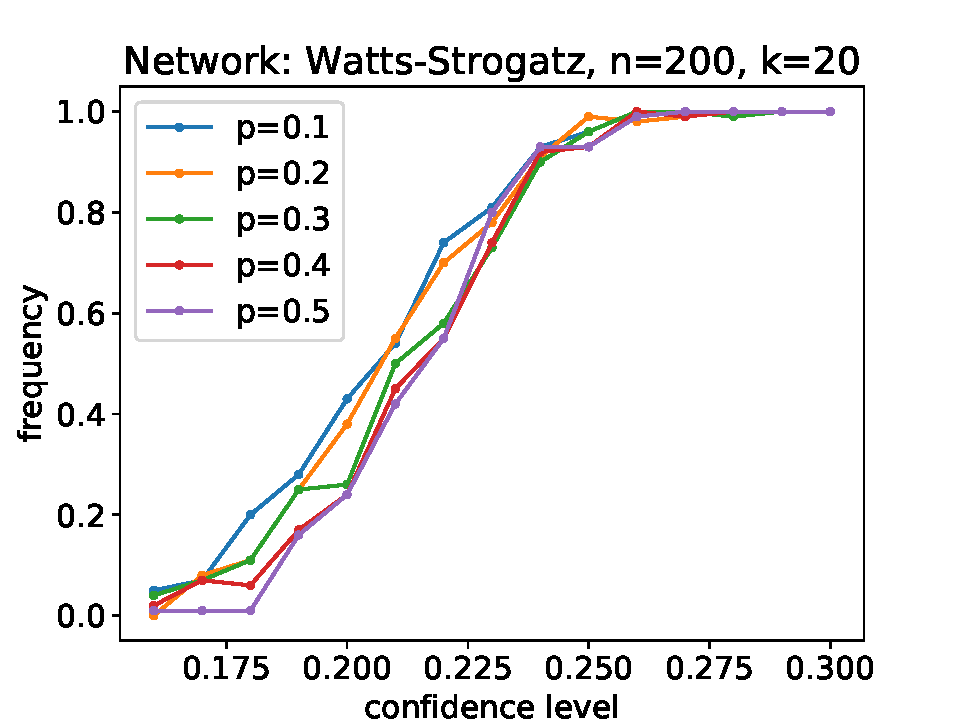
\includegraphics[width=\textwidth]{/home/arti/studia/python/praca_magisterska/plots/freq_consensus_ws_200_k=20.pdf}
            \caption{Watts--Strogatz: various $p$}
        \end{minipage}
        \hspace{0.5cm}
        \begin{minipage}[b]{0.45\linewidth}
            \centering
            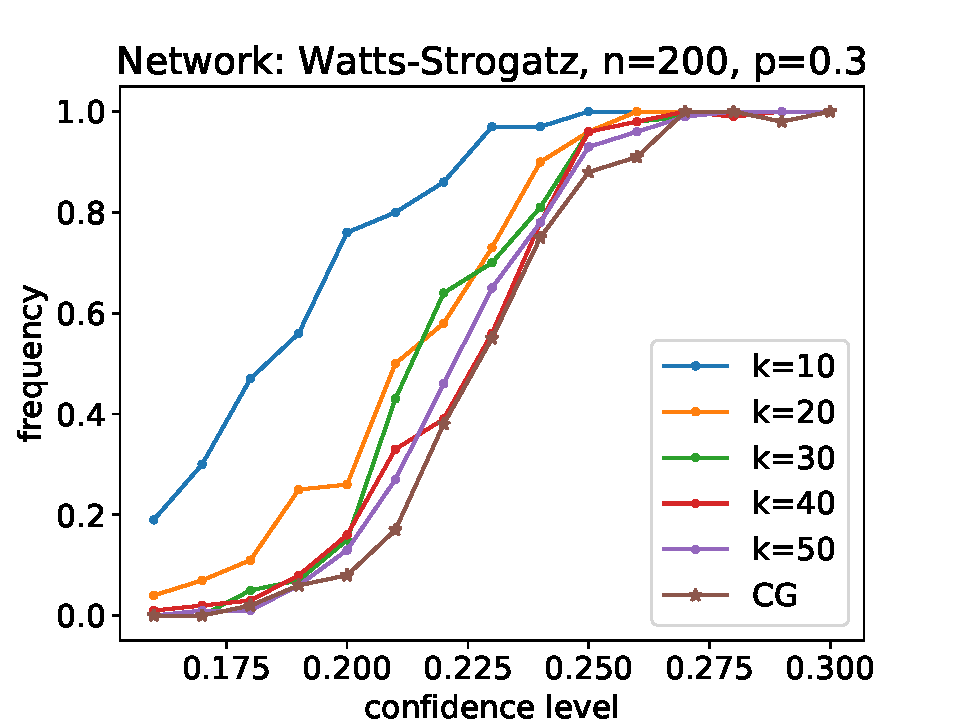
\includegraphics[width=\textwidth]{/home/arti/studia/python/praca_magisterska/plots/freq_consensus_ws_200_p=0,3.pdf}
			\caption{Watts--Strogatz: various $k$}
        \end{minipage}
    \caption{Frequency of reaching consensus}
    \end{figure}
\end{frame}

\begin{frame}
\frametitle{Consensus}
	\begin{figure}[ht]
		\begin{minipage}[b]{0.45\linewidth}
            \centering
            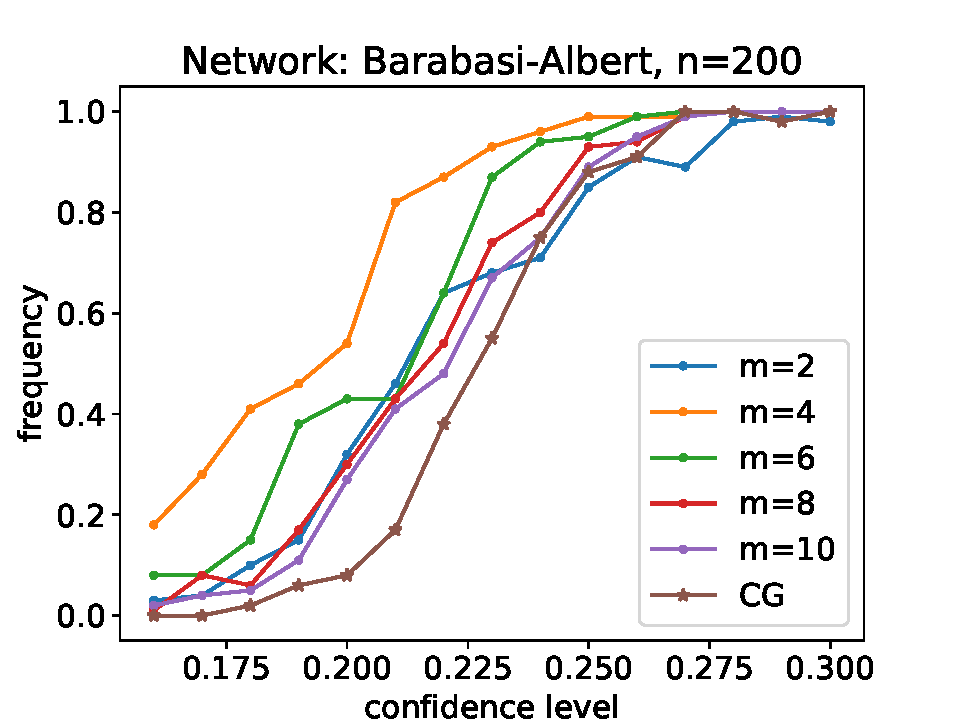
\includegraphics[width=\textwidth]{/home/arti/studia/python/praca_magisterska/plots/freq_consensus_ba_200.pdf}
            \caption{Barabasi--Albert: various $m$}
        \end{minipage}
        \hspace{0.5cm}
        \begin{minipage}[b]{0.45\linewidth}
            \centering
            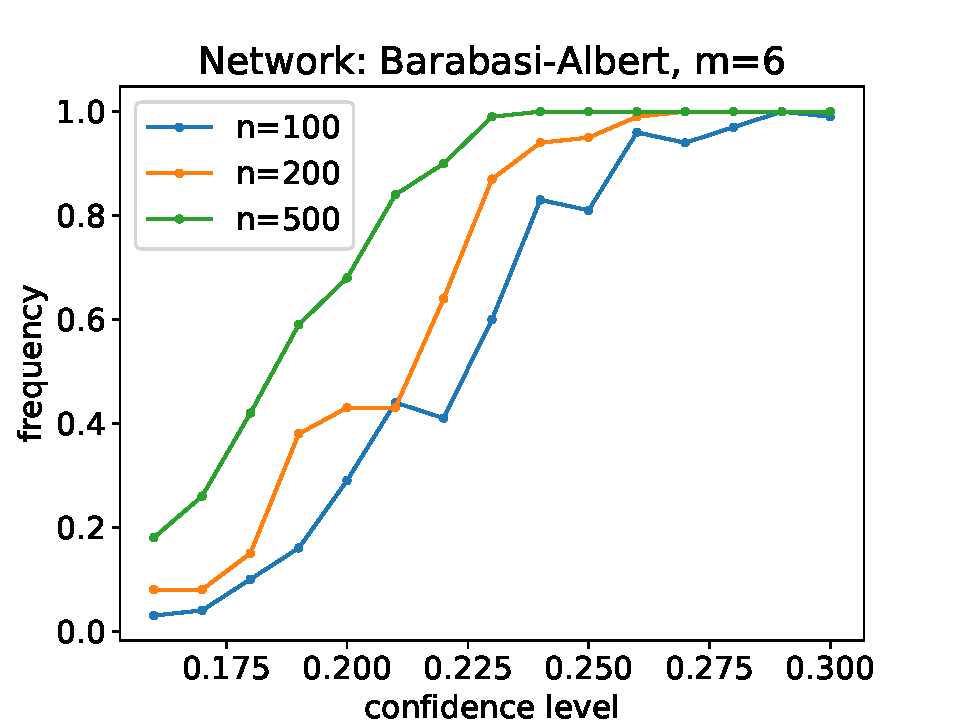
\includegraphics[width=\textwidth]{/home/arti/studia/python/praca_magisterska/plots/freq_consensus_ba_m=6.pdf}
			\caption{Barabasi--Albert: various $n$}
        \end{minipage}
    \caption{Frequency of reaching consensus}
    \end{figure}
\end{frame}

\begin{frame}
\frametitle{Consensus}
\begin{figure}[H]
		\centering
		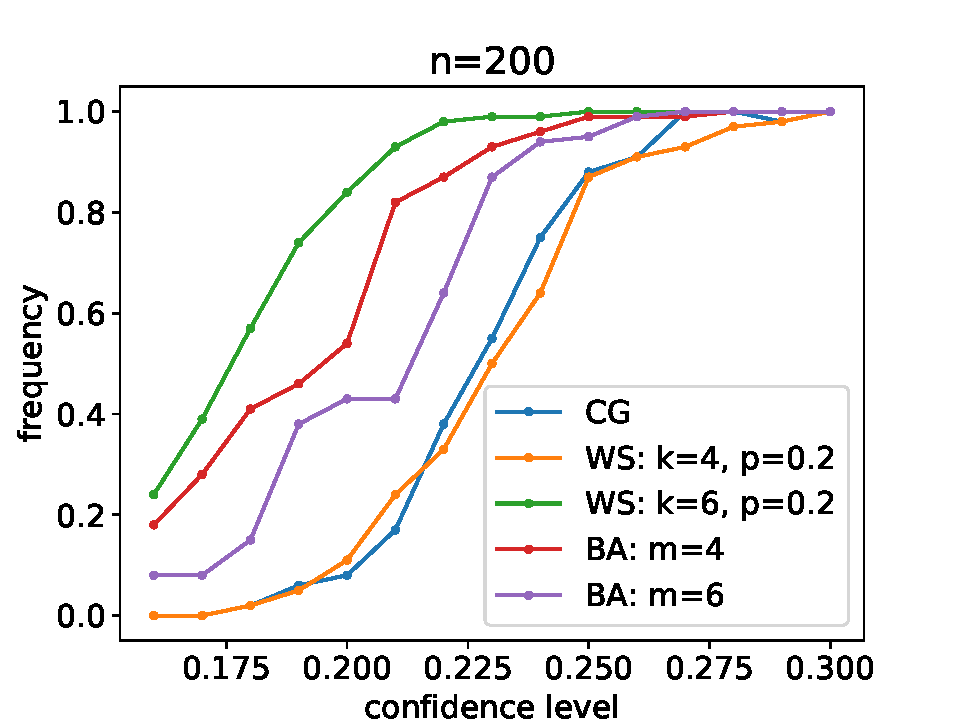
\includegraphics[width=.6\textwidth]{/home/arti/studia/python/praca_magisterska/plots/freq_consensus_compare.pdf}
		\caption{Frequency of reaching consensus: various networks}
\end{figure}
\end{frame}


\subsection{Relaxation time}

\begin{frame}
\frametitle{Relaxation time}
	\begin{figure}[ht]
		\begin{minipage}[b]{0.45\linewidth}
            \centering
            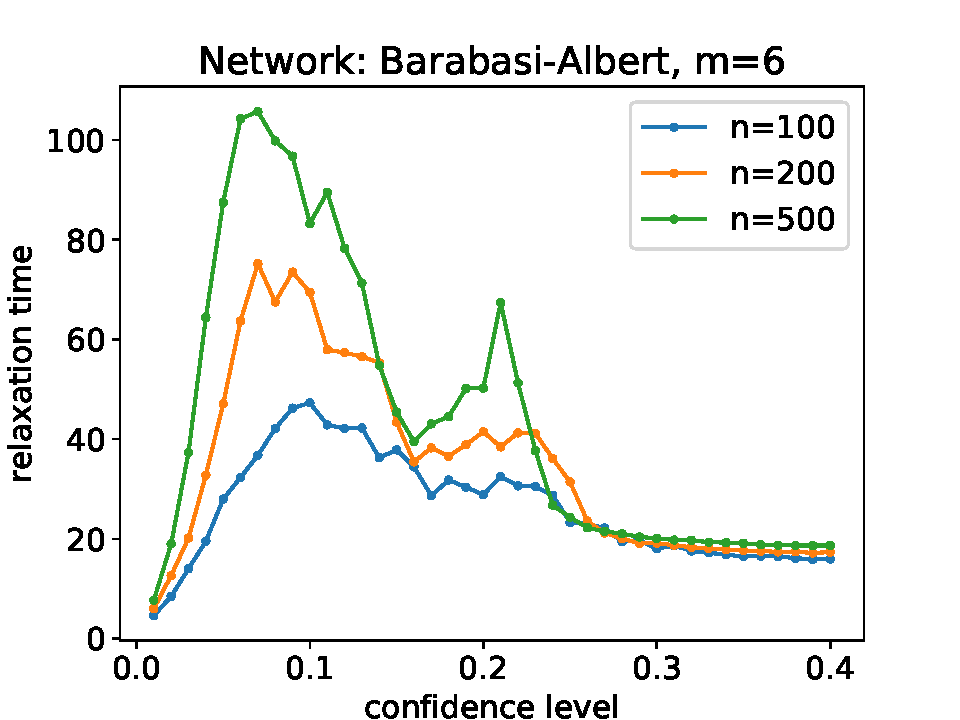
\includegraphics[width=\textwidth]{/home/arti/studia/python/praca_magisterska/plots/steps_Barabasi-Albert_m=6.pdf}
            \caption{Barabasi--Albert: various $n$}
        \end{minipage}
        \hspace{0.5cm}
        \begin{minipage}[b]{0.45\linewidth}
            \centering
            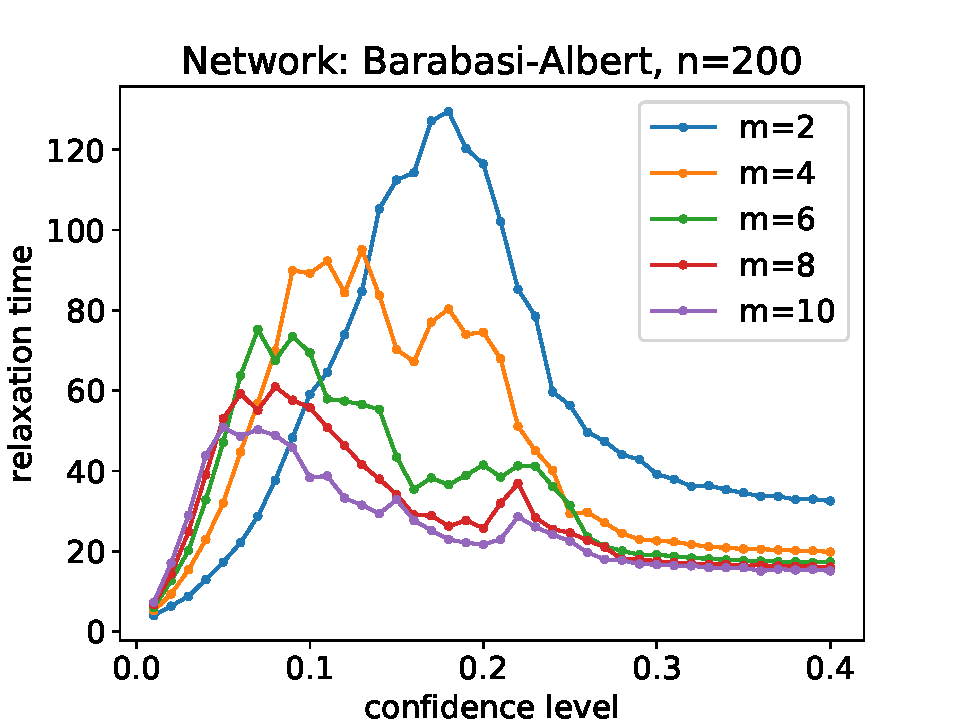
\includegraphics[width=\textwidth]{/home/arti/studia/python/praca_magisterska/plots/steps_Barabasi-Albert_n=200.pdf}
            \caption{Barabasi--Albert: various $m$}
        \end{minipage}
    \caption{Average relaxation time}
    \end{figure}
\end{frame}


\begin{frame}
\frametitle{Relaxation time}
	\begin{figure}[ht]
		\begin{minipage}[b]{0.45\linewidth}
            \centering
            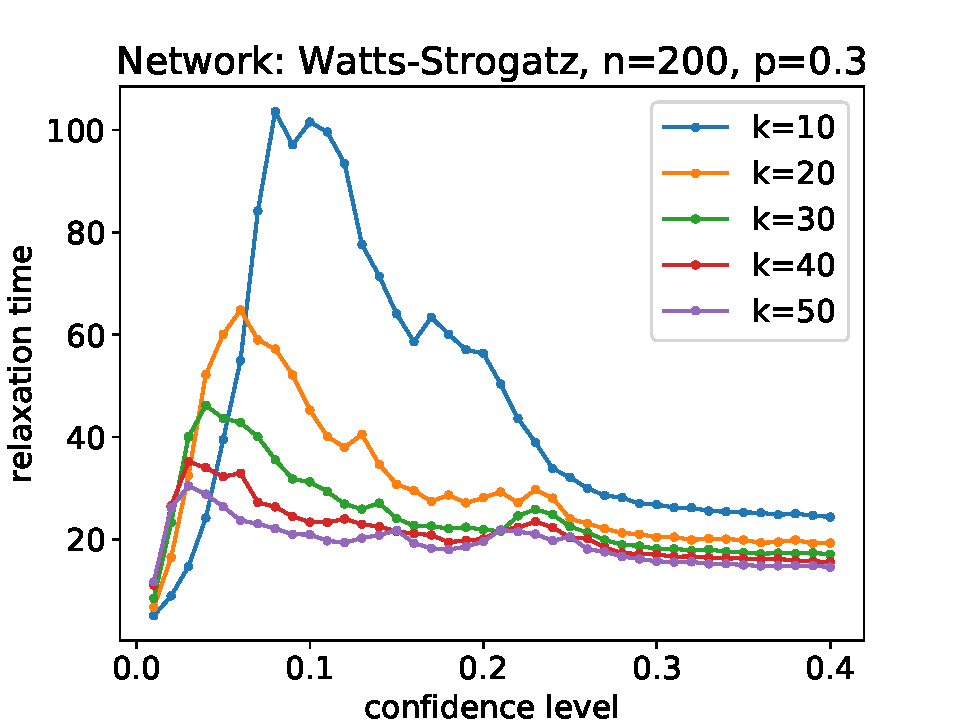
\includegraphics[width=\textwidth]{/home/arti/studia/python/praca_magisterska/plots/steps_Watts-Strogatz_n=200_p=0_3.pdf}
            \caption{Watts-Strogatz: various $k$}
        \end{minipage}
        \hspace{0.5cm}
        \begin{minipage}[b]{0.45\linewidth}
            \centering
            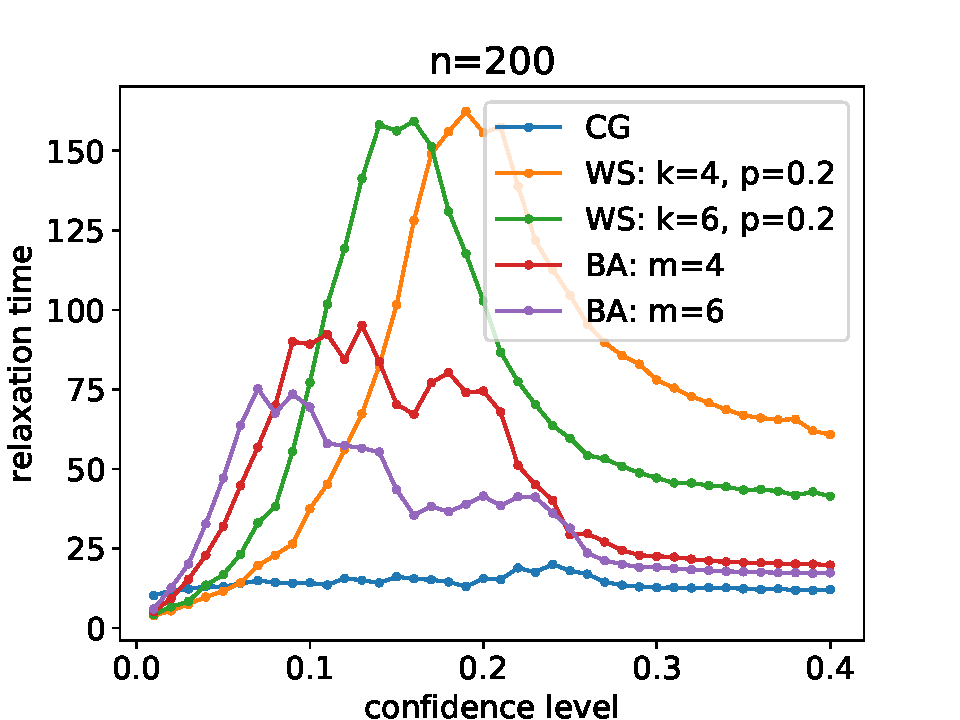
\includegraphics[width=\textwidth]{/home/arti/studia/python/praca_magisterska/plots/steps_various.pdf}
            \caption{Various networks}
        \end{minipage}
    \caption{Average relaxation time}
    \end{figure}
\end{frame}

\section{Conclusions}
\begin{frame}
\frametitle{Conclusions}
\begin{itemize}
	\item if underlying network is not well--connected, there are some agents who don't follow others opinion, usually their opinions are extreme (close to bounds)
	\item as confidence level is increasing, we go through three different states of opinion formation: fragmentarization, polarization and consensus
	\item weak--connected and strong--connected networks reach consensus less frequently than medium--connected
	\item opinion formation for not--centralized and week--connected (e.g. Watts--Strogatz with $k=4$) networks lead to big number of independent clusters
	\item consensus is reached more frequently for bigger networks
	\item wide--spread networks relax very slowly, strong--connected form stable formation the fastest
\end{itemize}
\end{frame}

\section{Literature}
\begin{frame}
\frametitle{Literature}
\begin{thebibliography}{1}


\bibitem{l1} Hegselmann, R. \& Krause, U. (2002). Opinion dynamics and bounded confidence: models, analysis and simulation. Journal of Artificial Societies and Social Simulation, 5(3)

\bibitem{l2} Claudio Castellano, Santo Fortunato, and Vittorio Loreto, Statistical physics of social dynamics, Rev. Mod. Phys. 81, 591 (2009)

\bibitem{l3} A. Jędrzejewski, K. Sznajd-Weron, J. Szwabiński, Mapping ,the q-voter model: From a single chain to complex networks, Physica A 446 (2016)

\end{thebibliography}
\end{frame}

\end{document}